\documentclass[https://www.overleaf.com/project/63761df255a8a9f4a15c3579
	letterpaper, % Paper size, specify a4paper (A4) or letterpaper (US letter)
	10pt, % Default font size, specify 10pt, 11pt or 12pt
]{CSUniSchoolLabReport}


\usepackage{verbatim}
\usepackage{fontawesome}
\usepackage{hyperref}
\usepackage[normalem]{ulem}
\usepackage{listings}
\usepackage{xcolor}
\definecolor{codegreen}{rgb}{0,0.6,0}
\definecolor{codegray}{rgb}{0.5,0.5,0.5}
\definecolor{codepurple}{rgb}{0.58,0,0.82}
\definecolor{backcolour}{rgb}{1,1,1}
\lstdefinestyle{mystyle}{
    backgroundcolor=\color{backcolour},   
    commentstyle=\color{codegreen},
    keywordstyle=\color{magenta},
    numberstyle=\tiny\color{codegray},
    stringstyle=\color{codepurple},
    basicstyle=\ttfamily\footnotesize,
    breakatwhitespace=false,         
    breaklines=true,                 
    captionpos=b,                    
    keepspaces=true,                 
    numbers=left,                    
    numbersep=5pt,                  
    showspaces=false,                
    showstringspaces=false,
    showtabs=false,                  
    tabsize=2
}

\lstset{style=mystyle}
\renewcommand\ULthickness{1.0pt}   %%---> For changing thickness of underline
\setlength\ULdepth{1.3ex}%\maxdimen ---> For changing depth of underline

%----------------------------------------------------------------------------------------
%	REPORT INFORMATION
%----------------------------------------------------------------------------------------


\begin{document}
    
    \begin{figure}[H] % [H] forces the figure to be placed exactly where it appears in the text
    	\centering % Horizontally center the figure
    	
\includegraphics[width=0.4\textwidth]{images/logo.png} % Include the figure
    \end{figure}
    
    \begin{center}
        \begin{tabular} {c}
            \Huge Universidad La Salle \\\\\\\\
            \huge Compiladores \\\\\\\\
            \LARGE Informe del Trabajo Parcial \\\\\\\\
            \huge Algoritmo LL1 \\\\\\\\
            \LARGE Karlo Emigdio Pacha Curimayhua \\\\\\\\
            \LARGE Sexto Semestre - Ingeniería de Software \\\\\\\\
            \LARGE 2023
          \end{tabular}
    \end{center}
    
    \begin{center}
    	\begin{tabular}{l r}
    	\end{tabular}
    \end{center}
    
    %----------------------------------------------------------------------------------------
    %	Introducción
    %----------------------------------------------------------------------------------------
    
    \section{Introducción }
    
    En muchos de los lenguajes actuales el tipo de declaración del código es algo compleja y a veces innecesariamente  "larga" como lo puede ser el '\(||\)' (or), en muchos lenguajes el símbolo '\(|\)' sólo se usa para la condición, sería más simple escribir sólo una vez el símbolo. 
    \\\\
    Este lenguaje busca simplificar la forma de escribir código, con el propósito de ahorrar algo de tiempo y para que el código sea más legible y ocupe menos espacio. Drachen Script se basa en lenguajes como: Python, Go, JavaScript y C\#. El objetivo principal es la comodidad.
    
    %----------------------------------------------------------------------------------------
    %	Especificación Léxica
    %----------------------------------------------------------------------------------------
    
    \section{Especificación Léxica}
    
    \subsection{Comentarios}
    En Drachen Script, los comentarios empiezan con el símbolo // y /**/ para comentarios multilinea. Estos deben estar dentro de una función o en el main \\
    
    \begin{lstlisting}
        // esto es un comentario de una linea
        /* comentario multilinea 
        mas lineas del comentario*/
    \end{lstlisting}
    
    %------------------------------------------------------------------
    \subsection{Identificadores}
    En Drachen Script, los identificadores empiezan con una letra (mayúscula o minúscula), le puede seguir un número, más letras o el subguión |. \\
    
    \begin{lstlisting}
        func MiFuncion (miParametro) {...}
        
        var MiIdentificador = 10,
        var mi_segundo_identificador = 20,
    \end{lstlisting}
    
    %------------------------------------------------------------------
    \subsection{Palabras clave}
    En Drachen Script, las palabras clave serán para estructuras como: if, while y for. Algunas otras se usarán para llamar a funciones como main(), read() o print(). Otras palabras reservadas serán para las funciones: func, exec y return. Finalmente para la declaración de variables y los tipos de booleanos: var, null, true y false. \\
    
    \begin{lstlisting}
    main() {
        var a = true,
        var b = exec MiFuncion(),
        if a {
            for i = 0, 10, 2 {
                print(i),
            }
        }
        return 0,
    }
    \end{lstlisting}
    
    %------------------------------------------------------------------
    \subsection{Operadores}
    En Drachen Script, los operadores serán: + (suma), - (resta), * (multiplicación) y / (división).
    Los operadores lógicos serán: == (igual), > (mayor),< (menor), <= (menor o igual), >= (mayor o igual), y != (diferente).\\
    
    \begin{lstlisting}
    main() {
        var a = true,
        var b = 10,
        if a == false {
        }
    
        if b < 11 {
        } 
    
        if a != false {
        }
    }
    \end{lstlisting}
    
    %------------------------------------------------------------------
    \subsection{Literales}
    En Drachen Script, los literales comparten similitud con la mayoría de lenguajes de programación actuales. \\
    
    \begin{lstlisting}
        var entero = 123,
        var flotante = 1.23,
        var cadena = "abc",
        var cadena2 = 'abc',
        var booleano = true,
        var nulo = null,
    \end{lstlisting}
    
    %------------------------------------------------------------------
    \section{Expresiones regulares}
    
    \begin{center}
        \begin{tabular}{| c | c |}
            \hline
                Token & Expresión Regular \\ 
            \hline
                Identifier & \([a-zA-Z]([a-zA-Z]|[0-9]|[\)|\(])*\) \\
                IntNumber & \([0-9]+\) \\
                FloatNumber & \([0-9]*(.)[0-9]+\) \\ 
                String & \(("|')([a-z]|[A-Z]|[0-9]|(\setminus n)|(\epsilon))*("|')\) \\ 
                Var & \('var'\) \\
                Plus & \(+\) \\ 
                Minus & \(-\) \\ 
                Times  & \(*\) \\ 
                Divide & \(/\) \\ 
                LParen & \((\) \\ 
                RParen & \()\) \\ 
                RKey & \(\{\) \\ 
                LKey & \(\}\) \\ 
                Equal & \(=\) \\ 
                Greater & \(>\) \\ 
                Less & \(<\) \\ 
                EqualEqual & \(==\) \\ 
                GreaterEqual & \(>=\) \\ 
                LessEqual & \(<=\) \\ 
                Diferent & \(!=\) \\ 
                While & \('while'\) \\ 
                For & \('for'\) \\ 
                If & \('if'\) \\ 
                Elif & \('elif'\) \\
                Else & \('else'\) \\
                Function & \('func'\) \\ 
                Execute & \('exec'\) \\ 
                Return & \('return'\) \\ 
                Main & \('main'\) \\
                Var & \('var'\) \\
                Print & \('print'\) \\
                Read & \('read'\) \\
                Null & \('null'\) \\
                Comment & \(//.*\) \\
                MultiComment & \verb|\/*([^*]||\verb|[\r\n]||\verb|(\*+([^*/]||\verb|[\r\n])))*\*+\/| \\
                Comma & \(,\) \\
                Or & \(|\) \\
                And & \(\&\) \\
            \hline
        \end{tabular}
    \end{center}

    %----------------------------------------------------------------------------------------
    %	Gramática
    %----------------------------------------------------------------------------------------
    
    \section{Gramática}
    
    La siguiente gramática cumple con las condiciones para ser una Gramática LL1, no es ambigua y está factorizada por la izquierda.
    
    \subsection{Gramática LL1}

        La siguiente gramática usa símbolos y el vacío es igual a: \verb|''|.
        \lstinputlisting[language=text]{codes/LL1.txt}

        \subsubsection{Ejemplo de Input LL1}
            \lstinputlisting[language=text]{codes/exampleLL1.ds}
        
    \subsection{Gramática LL1 - Parser}

        La siguiente gramática no usa símbolos, usa palabras, es lo más cercano a la tabla LL1 para parsear; el vacío es igual a: \verb|''|.
        \lstinputlisting[language=text]{codes/LL1e.txt}

        \subsubsection{Ejemplo de Input LL1 - Parser}
            \lstinputlisting[language=text]{codes/exampleLL1e.ds}

    %----------------------------------------------------------------------------------------
    %	Ejemplos de Código
    %----------------------------------------------------------------------------------------
    
    \section{Ejemplos de Código}
    
    \subsection{Ejemplos Aceptados}
    Los siguientes ejemplos fueron aceptados por el Algoritmo LL1 implementado.
        \subsubsection{Example.ds}
            \lstinputlisting[language=text]{codes/example.ds}

            \begin{figure}[H]
            	\centering
            	
\includegraphics[width=1\textwidth]{images/example.png}
                \caption{ Árbol Sintáctico Generado }
            \end{figure}
            
        \subsubsection{Example2.ds}
            \lstinputlisting[language=text]{codes/example2.ds}

            \begin{figure}[H]
            	\centering
            	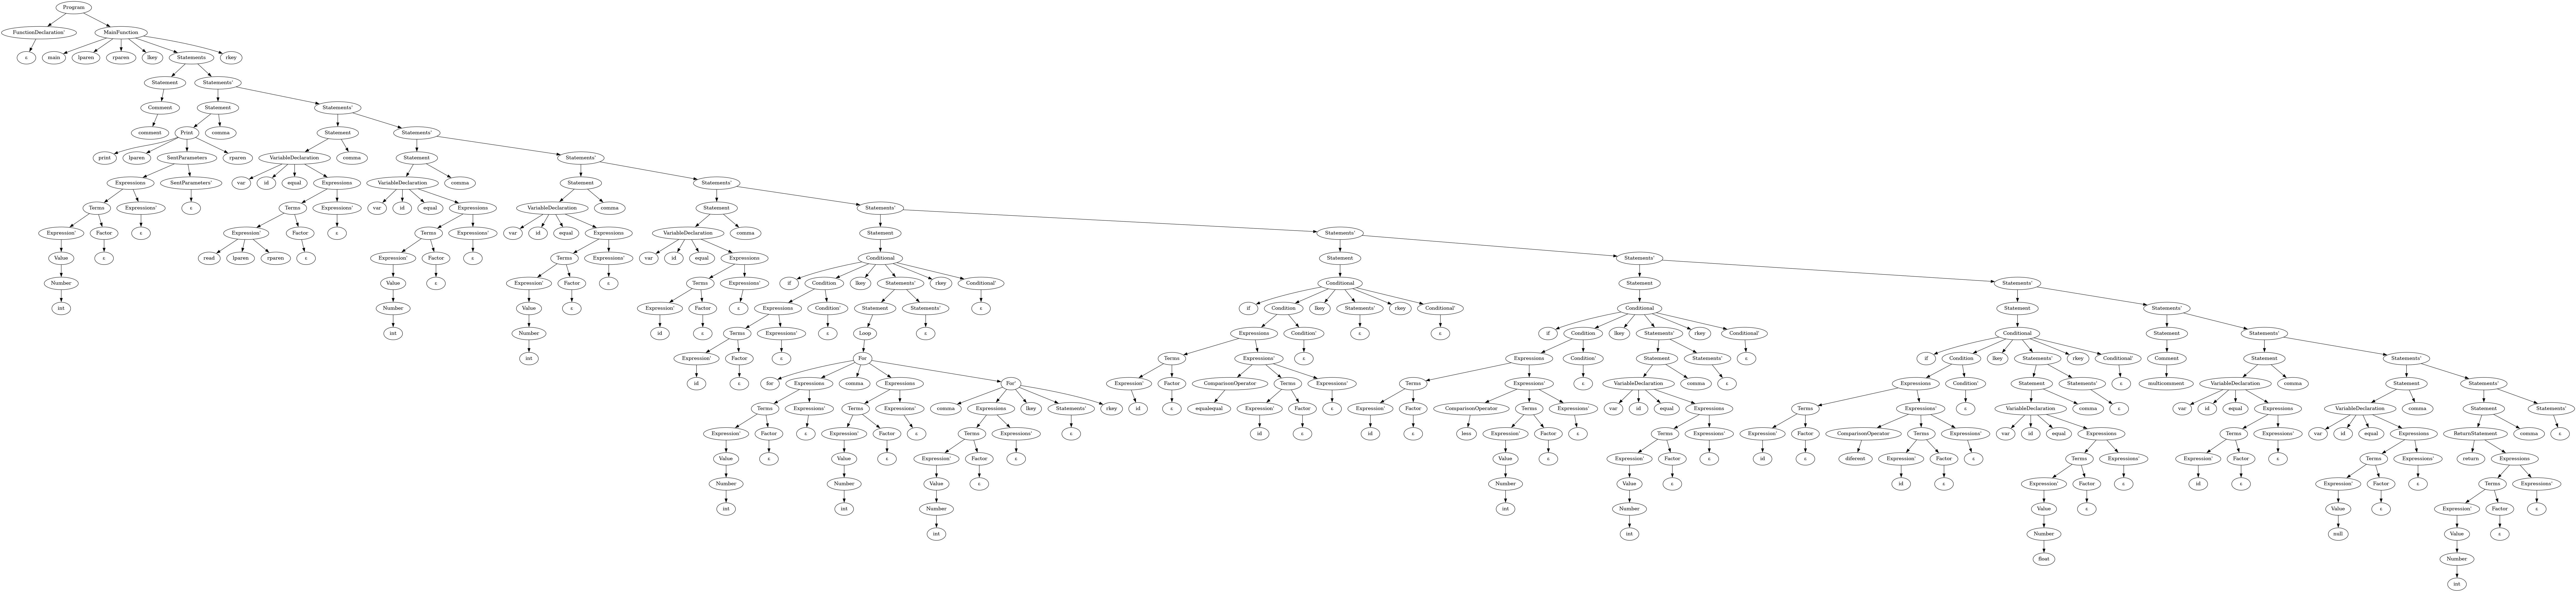
\includegraphics[width=1\textwidth]{images/example2.png}
                \caption{ Árbol Sintáctico Generado }
            \end{figure}
            
        \subsubsection{Example3.ds}
            \lstinputlisting[language=text]{codes/example3.ds}

            \begin{figure}[H]
            	\centering
            	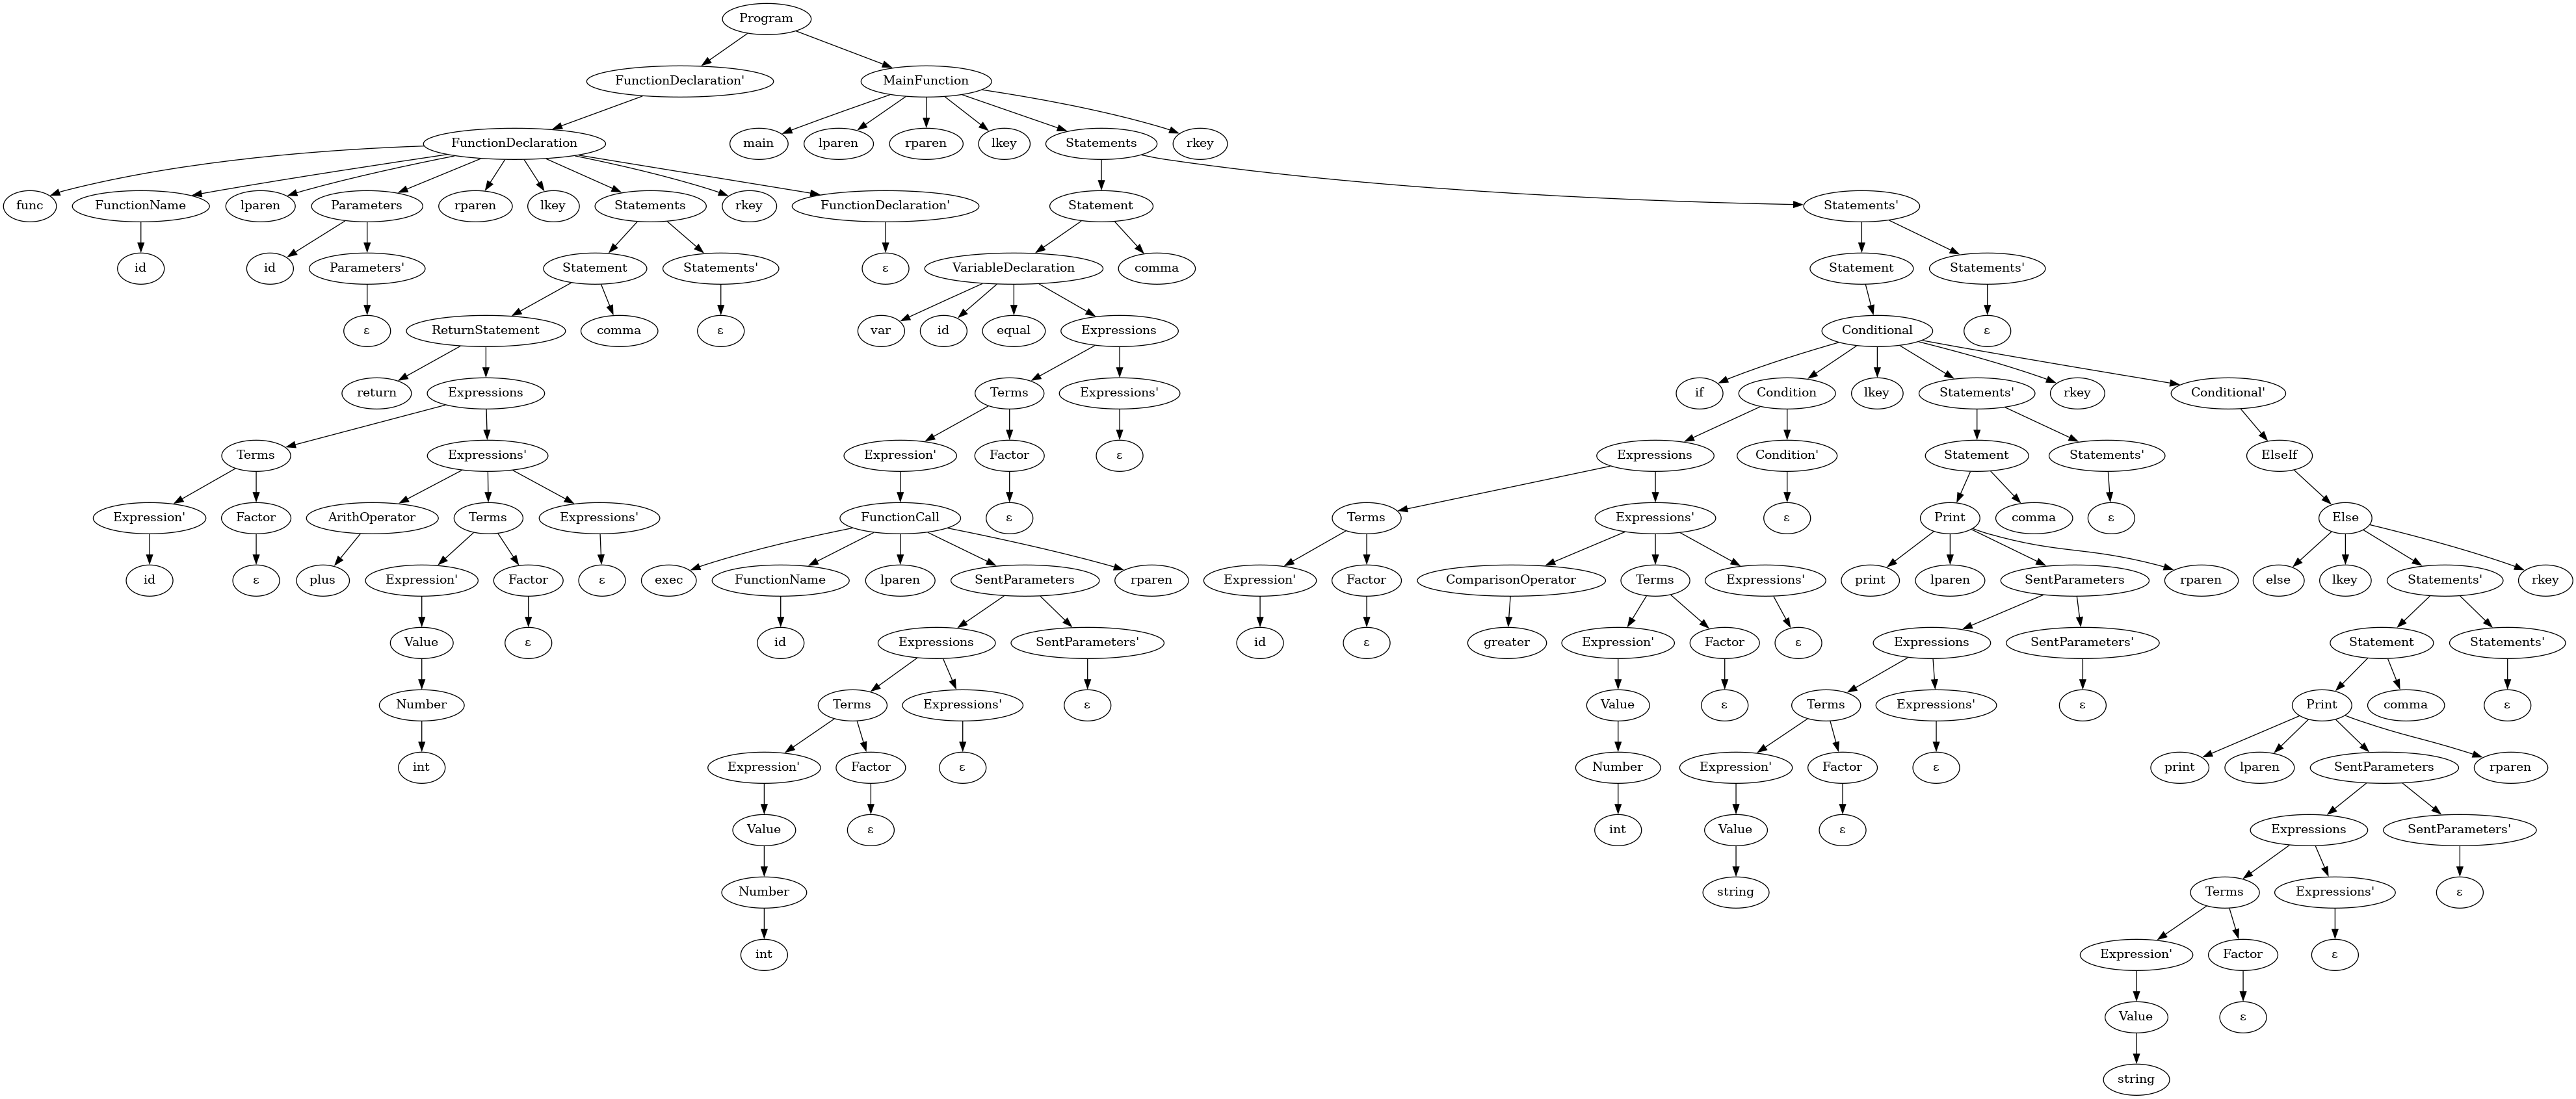
\includegraphics[width=1\textwidth]{images/example3.png}
                \caption{ Árbol Sintáctico Generado }
            \end{figure}

    \subsection{Ejemplos No Aceptados}
    Los siguientes ejemplos no fueron aceptados por el Algoritmo LL1 implementado.
        \subsubsection{BExample.ds}
            El primer error se encuentra en la línea 2, se espera que: "return a*a" termine con coma (,).
            \lstinputlisting[language=text]{codes/bexample.ds}
        \subsubsection{BExample2.ds}
            El primer error se encuentra en la línea 1, no se espera que haya un comentario fuera de una función o el main.
            \lstinputlisting[language=text]{codes/bexample2.ds}
        \subsubsection{BExample3.ds}
            El primer error se encuentra en la línea 6, no se espera que haya un id (AddOne) sin usar la palabra reservada func antes.
            \lstinputlisting[language=text]{codes/bexample3.ds}

        \begin{figure}[H]
            \centering
            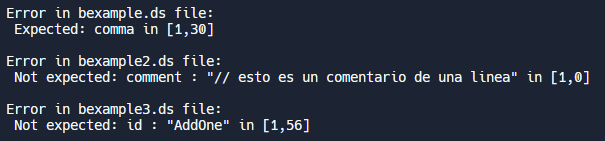
\includegraphics[width=1\textwidth]{images/Errors.png}
            \caption{ Errores de los 3 ejemplos no aceptados }
        \end{figure}


    %----------------------------------------------------------------------------------------
    %	Conclusiones
    %----------------------------------------------------------------------------------------
    
    \section{Conclusiones}
    
    El objetivo de este trabajo es crear un lenguaje que permita mayor comodidad al programador, con su forma de declarar tan fácil se espera crear un código legible y que sea fácil de identificar. Para facilitar ciertas labores lo mejor es usar herramientas web como LL1 Machine, y HTML-to-CSV.
    Durante la implementación del Algoritmo LL1 es mejor personalizar y agregar ciertas funciones para ver el progreso, en este caso se utilizaron funciones para generar archivos para la lista de Tokens (.out) y archivos para generear el árbol sintáctico (.dot), además de trabajar con el código dividido para tener un mejor rendimiento y entendimiento.\\\\

    %----------------------------------------------------------------------------------------
    \href{https://github.com/DAOBLUR/CompilersPractices/tree/main/partial} {\huge\faGithub \textbf{{Repositorio GitHub}} }
    
\end{document}